%-------------------------------------------------------------------------
% Design Project Input/Output Module Description
%-------------------------------------------------------------------------

\clearpage
\section{Temperature Input Module}
\label{sec-input-temperature}

This input module enables your IoT device to sense the temperature of
the environment using an easy-to-use temperature sensor. This may be
useful in environmental control systems, thermal protection, industrial
process control, fire alarms, power system monitors, cpu thermal
management, etc. The TMP36 temperature sensor contains an integrated
circuit with a single signal output lead. This signal's voltage rises
and falls, depending on the ambient temperature, at \wu{10}{mV} per
degree centigrade (Celsius).

A sample circuit and Arduino code is shown below to get you started.
There is no need for any extra components; we directly connect the
middle lead on the temperature sensor to an analog input on the Arduino.
Make sure the sensor's "flat end" is facing the correct direction (shown
in the diagram). If you point the flat end of the sensor to your left,
the top lead connects to power (the red wire), the middle lead is the
signal, and the bottom lead connects to ground (the black wire).

Since the analog reading from the temperature sensor is a digital value
between 0 and 1023, the example code scales this value to a range
between \wu{0--5}{V}, converts voltage to temperature, and then prints
the temperature in centigrade (Celsius) on the serial monitor, similar
to how we printed the analog reading from the grayscale sensor in Lab~2.
After setting up the circuit and programming the Arduino, open the
serial monitor and check the reported room temperature in degrees
centigrade (Celsius). Does the reading sound right? Experiment with the
sensor by changing the ambient temperature (e.g., with a hair dryer)
and see how warm or cool you can make it!

\vspace{0.1in}
\begin{minipage}[t]{0.49\tw}
  \vspace{0.6in}

  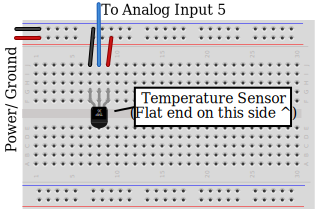
\includegraphics[width=\tw]{input-temperature-annotated.svg.pdf}
\end{minipage}
\hfill
\begin{minipage}[t]{0.49\tw}
  \vspace{0.1in}
  \begin{Verbatim}[gobble=3,fontsize=\small]
    int pin_temperature = A0;

    void setup() {
      Serial.begin(9600);
      pinMode( pin_temperature, INPUT );
    }

    void loop() {

      // Read temperature sensor and convert from
      // a 0 to 1023 digital range to 0 to 5 volts.

      float voltage =
        analogRead( pin_temperature ) * .004882814;

      // Convert from 10 mV per degree with 500
      // mV offset to degrees Celsius (i.e.,
      // temperature = (voltage-500mV) * 100).

      float temperature = (voltage - .5) * 100;

      Serial.println( temperature );
      delay(1000);
    }
  \end{Verbatim}
\end{minipage}
\vspace{0.1in}

%Questions:
